\chapter{Text characteristics analysis}

\epigraph{\textit{The main problem in working with language processing is that machine learning algorithms cannot work on the raw text directly. So, we need some feature extraction techniques to convert text into a matrix(or vector) of features.}}

In order to identify the authorship of an unknown text document using machine learning the document needs to be quantified first. The simple and natural way to characterize a document is to consider it as a sequence of tokens grouped into sentences where each token can be one of the three: word, number, punctuation mark.
To quantify the overall writing style of an author, stylometric features are defined and studied in different domains. Mainly, computations of stylometric features can be categorized into five groups as lexical, character, semantic, syntactic, and application specific features. Lexical and character features mainly considers a text document as a sequence of word tokens or characters, respectively. This makes it easier to do computations compared to other features. On the other hand, syntactic and semantic features require deeper linguistic analysis and more computation time. Application specific features are defined based on the text domains or languages. These five features are studied and the methods to extract them are also provided for interested readers.
Moreover there's a sixth characteristic regarding only hand-written text, which was used for years in the past and it's still studied nowadays \cite{mironovsky2018graphological}, which is the \textit{graphological analysis}.
Although the problem of recognition of handwriting text is still far from its final solution, in this work, we will focus only on the first 5 characteristics because the main focus since the digitalization era has been on studies of digital text characteristics analysis.

\section{Character Features}

Based on these features a sentence consists of a characters sequence. Some of the character-level features are alphabetic characters count, digit characters count, uppercase and lowercase character counts, letter and character n-gram frequencies. This type of feature extraction techniques has been found quite useful to quantify the writing style.\cite{grieve2007quantitative}
A more practical approach in character-level features are the extraction of n-gram characters. This procedure of extracting such features are language independent and require less complex toolboxes. On the other hand, comparing to word n-grams approach the dimensional of these approaches are vastly increased and it has a curse of dimensional problem. A simple way of explaining what a character n-grams could be with the following example: assume that a word “thesis” is going to be represented by 2-gram characters. So, the resulting sets of points will be {\enquote{th}, \enquote{he}, \enquote{es}, \enquote{si}, \enquote{is}}.\\
A simple python algorithm is shown in \ref{lst:CharNGramSplit}:\\

\begin{lstlisting}[frame=none,caption={Split word into character n-grams, parametric on n.},captionpos=b,label=lst:CharNGramSplit]
\end{lstlisting}
\begin{python}
	def get_char_n_gram(text, n=2):
		"""Convert text into character n-grams list"""
		return [text[i:i+n] for i in range(len(text)-n+1)]
	
	# Examples character 2-grams
	
	print(get_char_n_gram("thesis"))
	>>Out: ['th', 'he', 'es', 'si', 'is']
	
	print(get_char_n_gram("student", n=3))
	>>Out: ['stu', 'tud', 'ude', 'den', 'ent']
\end{python}


In \cite{sapkota2015not} 10 character n-grams categories have been identified, being proven as the most successful feature in both single-domain and cross-domain Authorship Attribution.\\
These 10 categories are grouped into 3 groups: Affix n-grams, Word n-grams, Punctuation n-grams.

\subsection{Affix n-grams}
Character n-grams are generally too short to represent any deep syntax, but some of them can reflect morphology to some degree. In particular, the following affix-like features are extracted by looking at n-grams that begin or end a word:

\begin{itemize}
	\item \textbf{prefix}: A character n-gram that covers the first n characters of a word that is at least n+1 characters long.
	\item \textbf{suffix}: A character n-gram that covers the last n characters of a word that is at least n + 1 characters long.
	\item \textbf{space-prefix}: A character n-gram that begins with a space.
	\item \textbf{space-suffix}: A character n-gram that ends with a space.
\end{itemize}

\subsection{Word n-grams}
While character n-grams are often too short to capture entire words, some types can capture partial
words and other word-relevant tokens. There's a distinction among:

\begin{itemize}
	\item \textbf{whole-word}: A character n-gram that covers all characters of a word that is exactly n characters long.
	\item \textbf{mid-word}: A character n-gram that covers n characters of a word that is at least n + 2 characters long, and that covers neither the first nor the last character of the word.
	\item \textbf{multi-word}: N -grams that span multiple words, identified by the presence of a space in the middle of the n-gram.
\end{itemize}

\subsection{Punctuation n-grams}

The main stylistic choices that character n-grams can capture are the author’s preferences for particular patterns of punctuation. The following features characterize punctuation by its location in the n-gram.

\begin{itemize}
	\item \textbf{beg-punct}: A character n-gram whose first character is punctuation, but middle characters are not.
	\item \textbf{mid-punct}: A character n-gram with at least one punctuation character that is neither the first nor the last character.
	\item \textbf{end-punct}: A character n-gram whose last character is punctuation, but middle characters are not.
\end{itemize}

\begin{table}[h!]
	\begin{center}  
		\caption[Example of the \textit{n}-gram categories (n=3)]{Example of the \textit{n}-gram categories (n=3) for the sentence: \textit{The actors wanted to see if the pact seemed like an old-fashioned one.} \\ 
			The \textit{n}-grams that appear in more than one category are in bold.} 
		\label{tab:examplesngram}
		%\resizebox{\linewidth}{!}{  %
		\begin{tabular}{|c | c |}
			\hline 
			\textbf{Category} & \textbf{Category n-grams} \\
			\hline \hline
			prefix & \textbf{act} wan pac \textbf{see} lik fas \\ \hline
			suffix & ors ted \textbf{act} med ike ned \\ \hline
			space-prefix & \_ac \_wa \_to \_se \_if \_th \_pa \_li \_an \_ol \_on \\ \hline
			space suffix & he\_ rs\_ ed\_ to\_ ee\_ if\_ ct\_ ke\_ an\_ \\ \hline
			whole-word & The \textbf{see} the old \textbf{one} \\ \hline
			mid-word & cto tor ant nte eem eme ash shi hio ion \textbf{one} \\ \hline
			multi-word & e\_a s\_w d\_t o\_s e\_i f\_t e\_p t\_s d\_l n\_o d\_o \\ \hline
			beg-punct & -fa \\ \hline
			mid-punct & d-f \\ \hline
			end-punct & ld- ne. \\ \hline
			%\bottomrule 
		\end{tabular} 
		%}
	\end{center}
\end{table}


\paragraph{}
In \autoref{tab:examplesngram} we can see an example of the n-gram categories ($ n = 3 $) for the sentence \textit{\enquote{The actors wanted to see if the pact seemed like an old-fashioned one.}}. 
In \cite{sapkota2015not} they've observed that in their data almost 80\% of the n-grams in the punct-beg and punct-mid categories contain a space. They stated that \enquote{this tight coupling of punctuation and spaces is due to the rules of English orthography: most punctuation marks require a space following them}. The 20\% of n-grams that have punctuation but no spaces correspond mostly to the exceptions to this rule: quotation marks, mid-word hyphens, etc.
The authors of \cite{sapkota2015not} conducted an experiment on Reuters Corpus Volume 1 (RCV1) dataset both the \textit{CCAT\_10 split} and the \textit{CCAT\_50 split}\footnote{CCAT\_10/CCAT\_50 split on RCV1 dataset is the selection of the 10/50 most prolific authors belonging to the Corporate/Industrial Category (CCAT)}. They've also used the Guardian dataset as a cross-domain authorship attribution experiment. In their work they stated that for the single-domain the top four categories for authorship attribution are: \textit{prefix}, \textit{suffix}, \textit{space-prefix} and \textit{mid-word}. On the other hand, for cross-domain authorship attribution the top four categories have been proven to be: \textit{prefix}, \textit{space-prefix}, \textit{beg-punct} and \textit{mid-punct}.
For both single-domain and cross-domain authorship attribution, \textit{prefix} and \textit{space-prefix} are strong features, and are generally better than the \textit{suffix} features, perhaps because authors have more control over prefixes in English,
while suffixes are often obligatory for grammatical reasons. For cross-domain authorship attribution, \textit{beg-punct} and \textit{mid-punct} they found to be the top features, likely because an author’s use of punctuation is consistent even when the topic
changes. For single-domain authorship attribution, \textit{mid-word} was also
a good feature, probably because it captured lexical information that correlates with authors’ preferences towards writing about specific topic.

\section{Lexical Features}

Lexical features relate to the words or vocabulary of a language. It is the very plain way of representing a sentence structure that consists of words, numbers, punctuation marks. These features are very first attempts to attribute authorship in earlier studies \cite{fox2012statistical}, \cite{argamon2005measuring}, \cite{stanko2013whose}. The main advantage of Lexical features is that it is universal and can be applied to any language easily. These features consist of bag of words representation, word N-grams, vocabulary richness, number of punctuation marks, average number of words in a sentence, and many more. Even though the number of lexical features can vary a lot, not all of them are good for every authorship attribution problem. That is why, it is important to know how to extract these features and try out different combinations on different classifiers.

\subsection{Bag of Words}
It is the representation of a sentence with frequency of words. It is a simple and efficient solution but it disregards word-order information.
At the very beginning, we applied this representation to our datasets, using the already implemented $CountVectorizer$ from $sklearn.feature\_extraction.text$. We gave this hyper-parameter to the function:
\begin{itemize}
	\item \textbf{max\_df}=0.8
	\item \textbf{max\_features}=10000
	\item \textbf{min\_df}=0.02
	\item \textbf{ngram\_range}=(1, 2)
\end{itemize}
In the approach, for each text fragment the number of instances of each unique word is found to create a vector representation of word counts. We capped the max number of features to 10'000 words and discarding the words with a higher frequency of 0.8 across the document and a lower frequency of 0.02. We've also taken into account both single word and word bi-grams. In order to give the reader a better perspective of the impact of this process for the task of authorship attribution, we choose two among the top ten most prolific authors in the RCV1 dataset: \textit{David Lawder} and \textit{Alexander Smith}.
In \autoref{fig:chartRCV1Top2Authors} we can see the number of documents written by the two selected authors in the RCV1 corpus for the \textit{CCAT} topic.

\begin{figure}[ht]
	\centering
	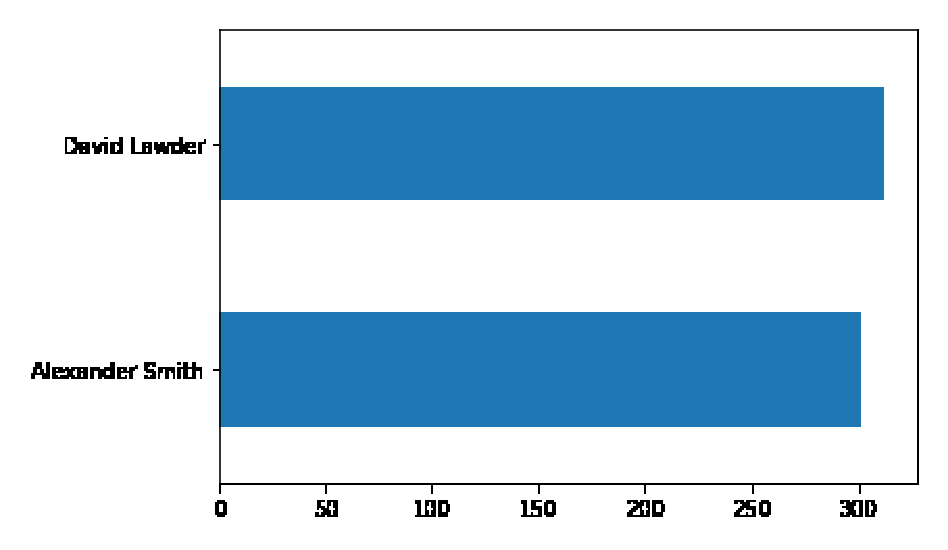
\includegraphics[width=1.0\textwidth, height=.8\textheight, keepaspectratio]{top_2_authors_rcv1_ccat}
	\caption[Number of documents for 2 authors in Reuters Corpus]{The number of documents written by David Lawder and Alexander Smith in the Reuters Corpus for the \textit{CCAT} topic.}
	\label{fig:chartRCV1Top2Authors}
\end{figure}

With a simple snippet of python code shown in \ref{lst:MostCommonWords}, we can get the most common words for an author across all the documents we gathered in the dataset.

\begin{lstlisting}[frame=none,caption={Top 20 most common words in a document or a collection of document by the same author.},captionpos=b,label=lst:MostCommonWords]
\end{lstlisting}
\begin{python}
	from collections import Counter
	
	def get_most_common_words_in_df(df, n=20):
		"""Split a collection of document in single word and order by frequencies across all documents"""
		most_common_words = Counter(" ".join(df["articles"]).split()).most_common(n)
		return most_common_words
\end{python}
\begin{python}	
	# Examples
	
	# 1. Top 20 words with their frequency for every document written by David Lawder
	
	print(get_most_common_words_in_df(dataset[dataset['author']=='David Lawder']))
	>>Out: [('the', 7844), ('to', 5133), ('of', 3875), ('and', 3746), ('a', 3719), ('in', 3552), ('said', 1749), ('that', 1720), ('for', 1574), ('GM', 1453), ('on', 1286), ('at', 1267), ('its', 1153), ('The', 1098), ('with', 990), ('is', 957), ('it', 897), ('will', 875), ('by', 868), ('from', 824)]
	
	# 2. Top 20 words without their frequency for every document written by David Lawder
	
	print([m[0] for m in get_most_common_words_in_df(dataset[dataset['author']=='David Lawder'])])
	>>Out: ['the',
			'to',
			'of',
			'and',
			'a',
			'in',
			'said',
			'that',
			'for',
			'GM',
			'on',
			'at',
			'its',
			'The',
			'with',
			'is',
			'it',
			'will',
			'by',
			'from']
	
\end{python}

\begin{figure}[ht]
	\centering
	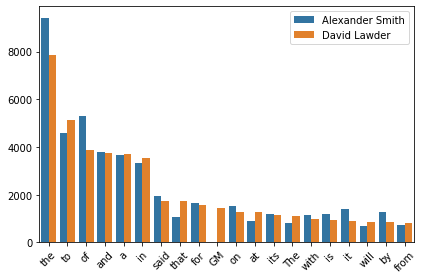
\includegraphics[width=1.0\textwidth, height=.8\textheight, keepaspectratio]{rcv1_top20_words_alexander_smith_vs_david_lawder}
	\caption[David Lawder vs Alexander Smith top 20 words]{Frequency usage of the top 20 words used in the RCV1 corpus by David Lawder, compared to the frequencies of the same words in the corpus by Alexander Smith.}
	\label{fig:chartRCV1ALvsDL}
\end{figure}

\begin{figure}[ht]
	\centering
	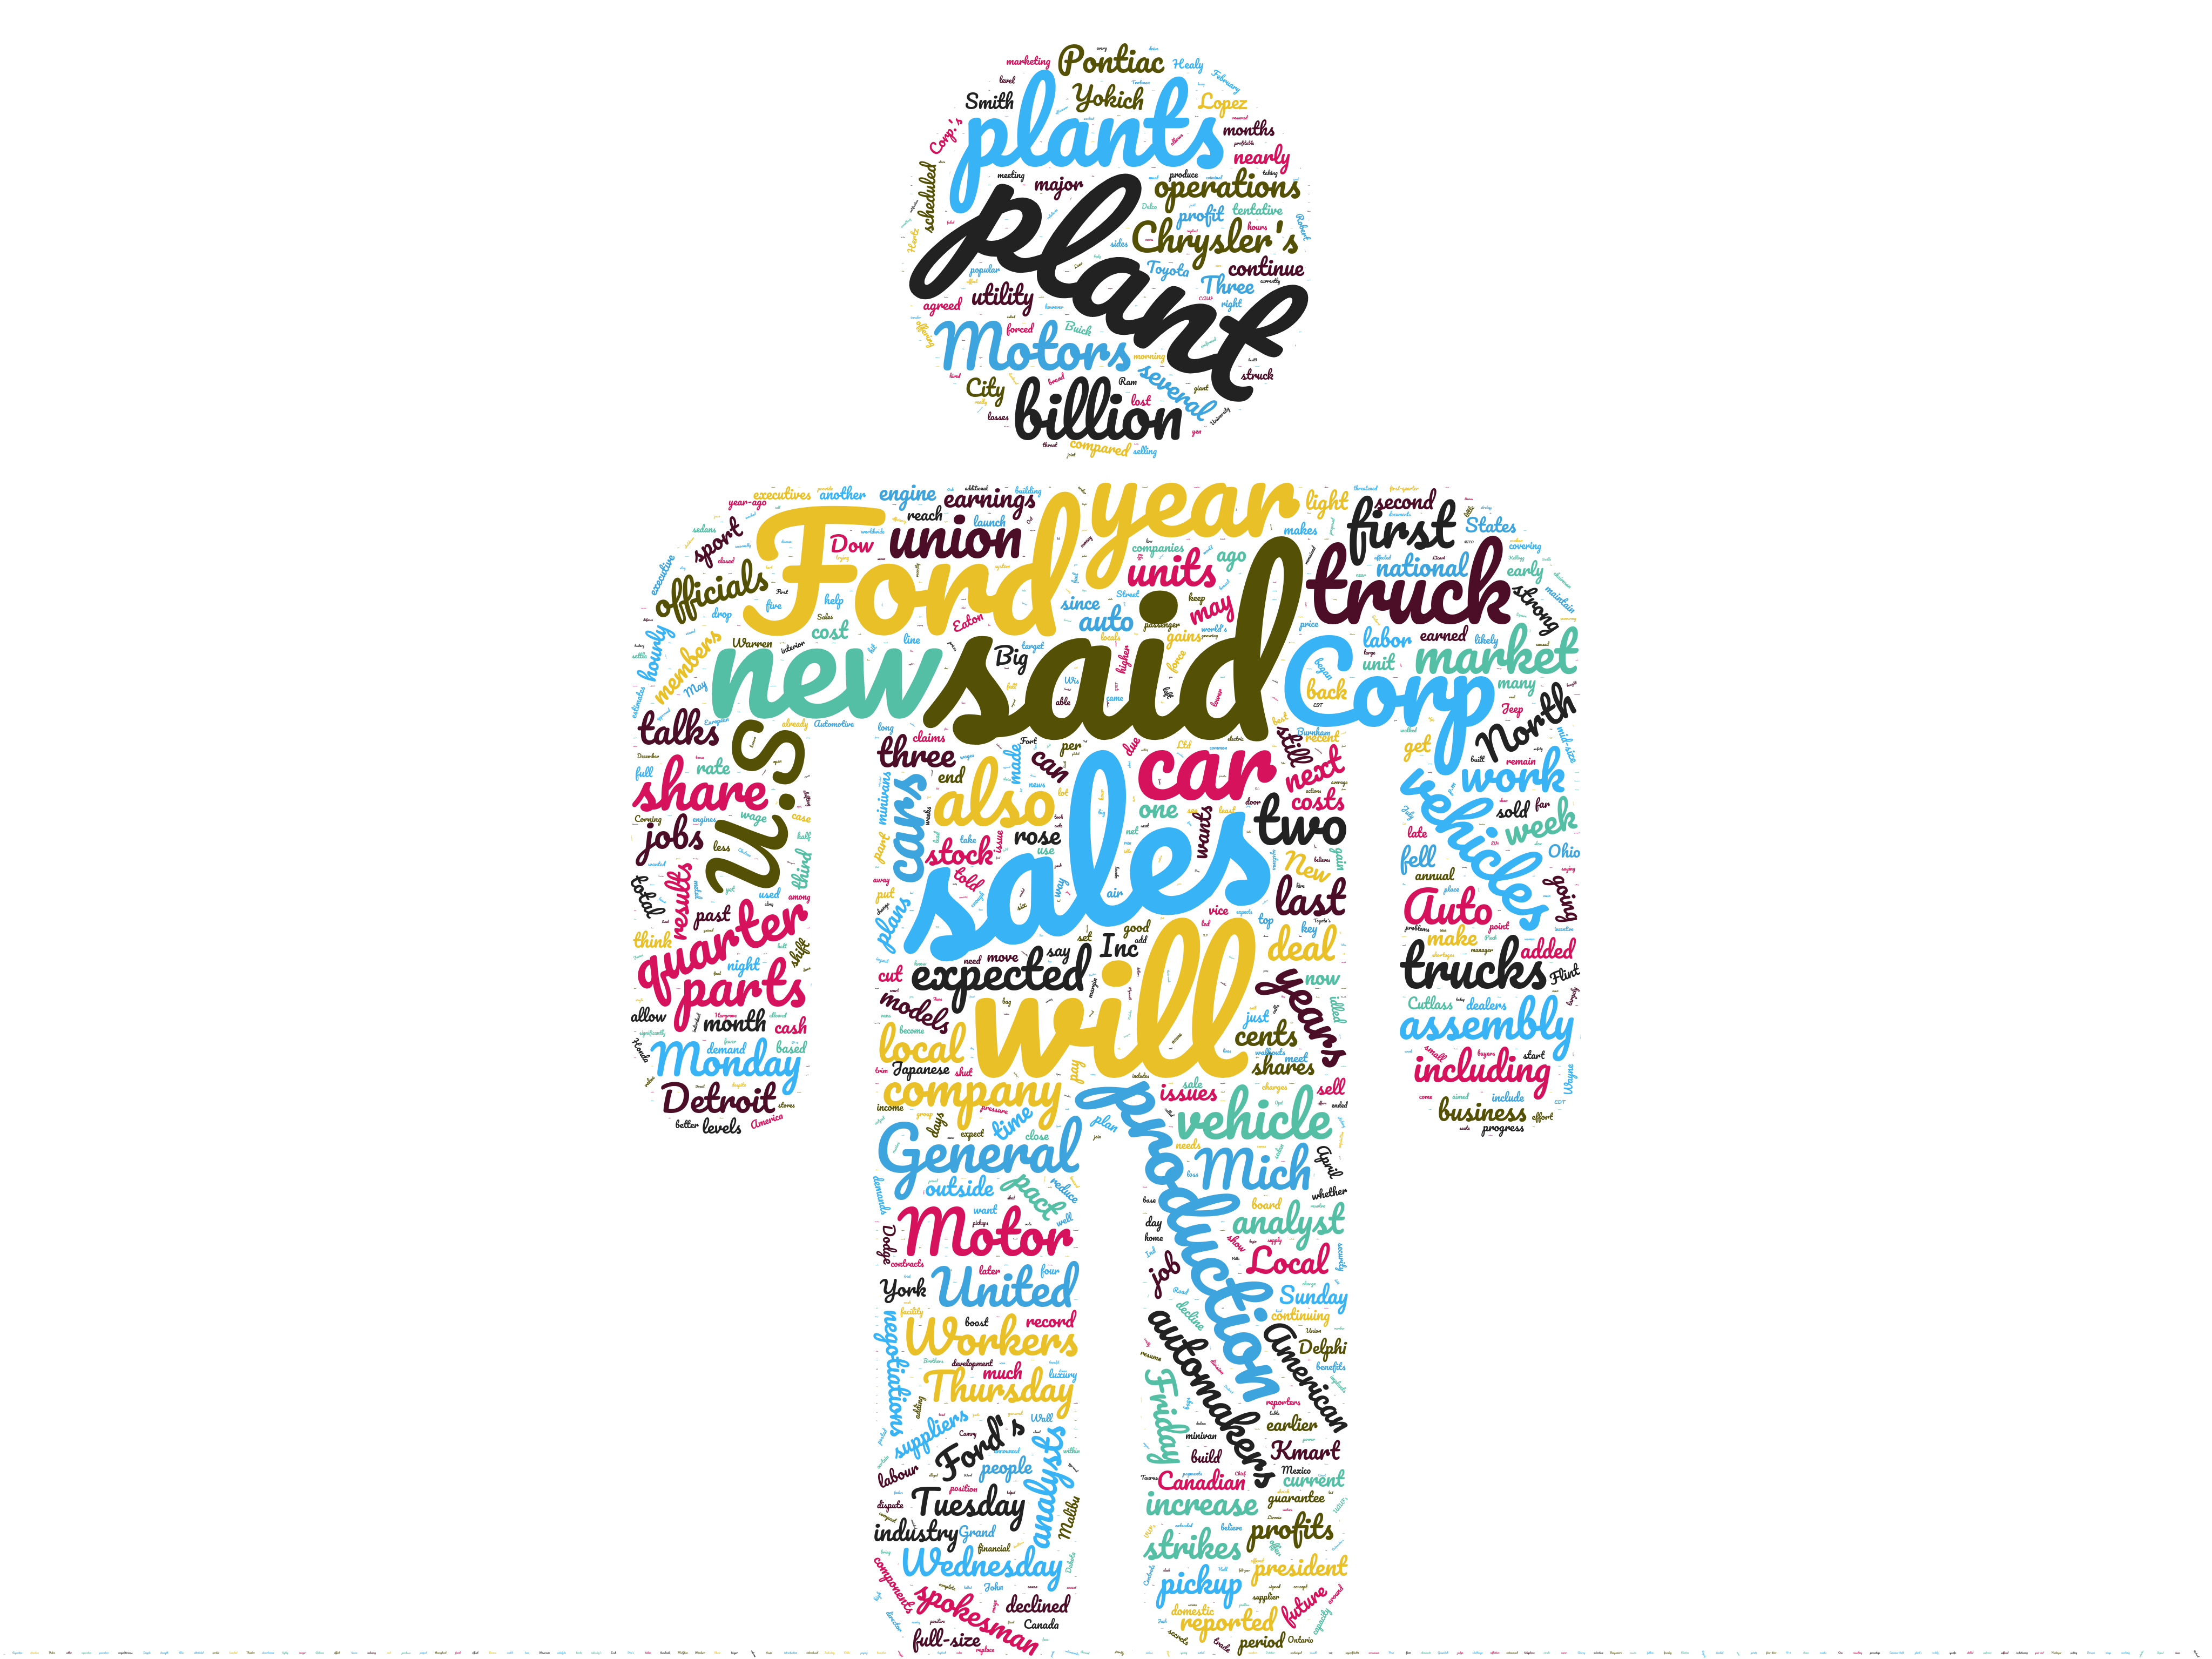
\includegraphics[width=.8\textwidth, height=.6\textheight, keepaspectratio]{David_Lawder_wordcloud}
	\caption[David Lawder WordCloud in Reuters Corpus]{Image Generated on \href{wordclouds.com} for every word in Reuters Corpus data for the documents written by David Lawder.}
	\label{fig:wordcloudDL}
\end{figure}

\begin{figure}[ht]
	\centering
	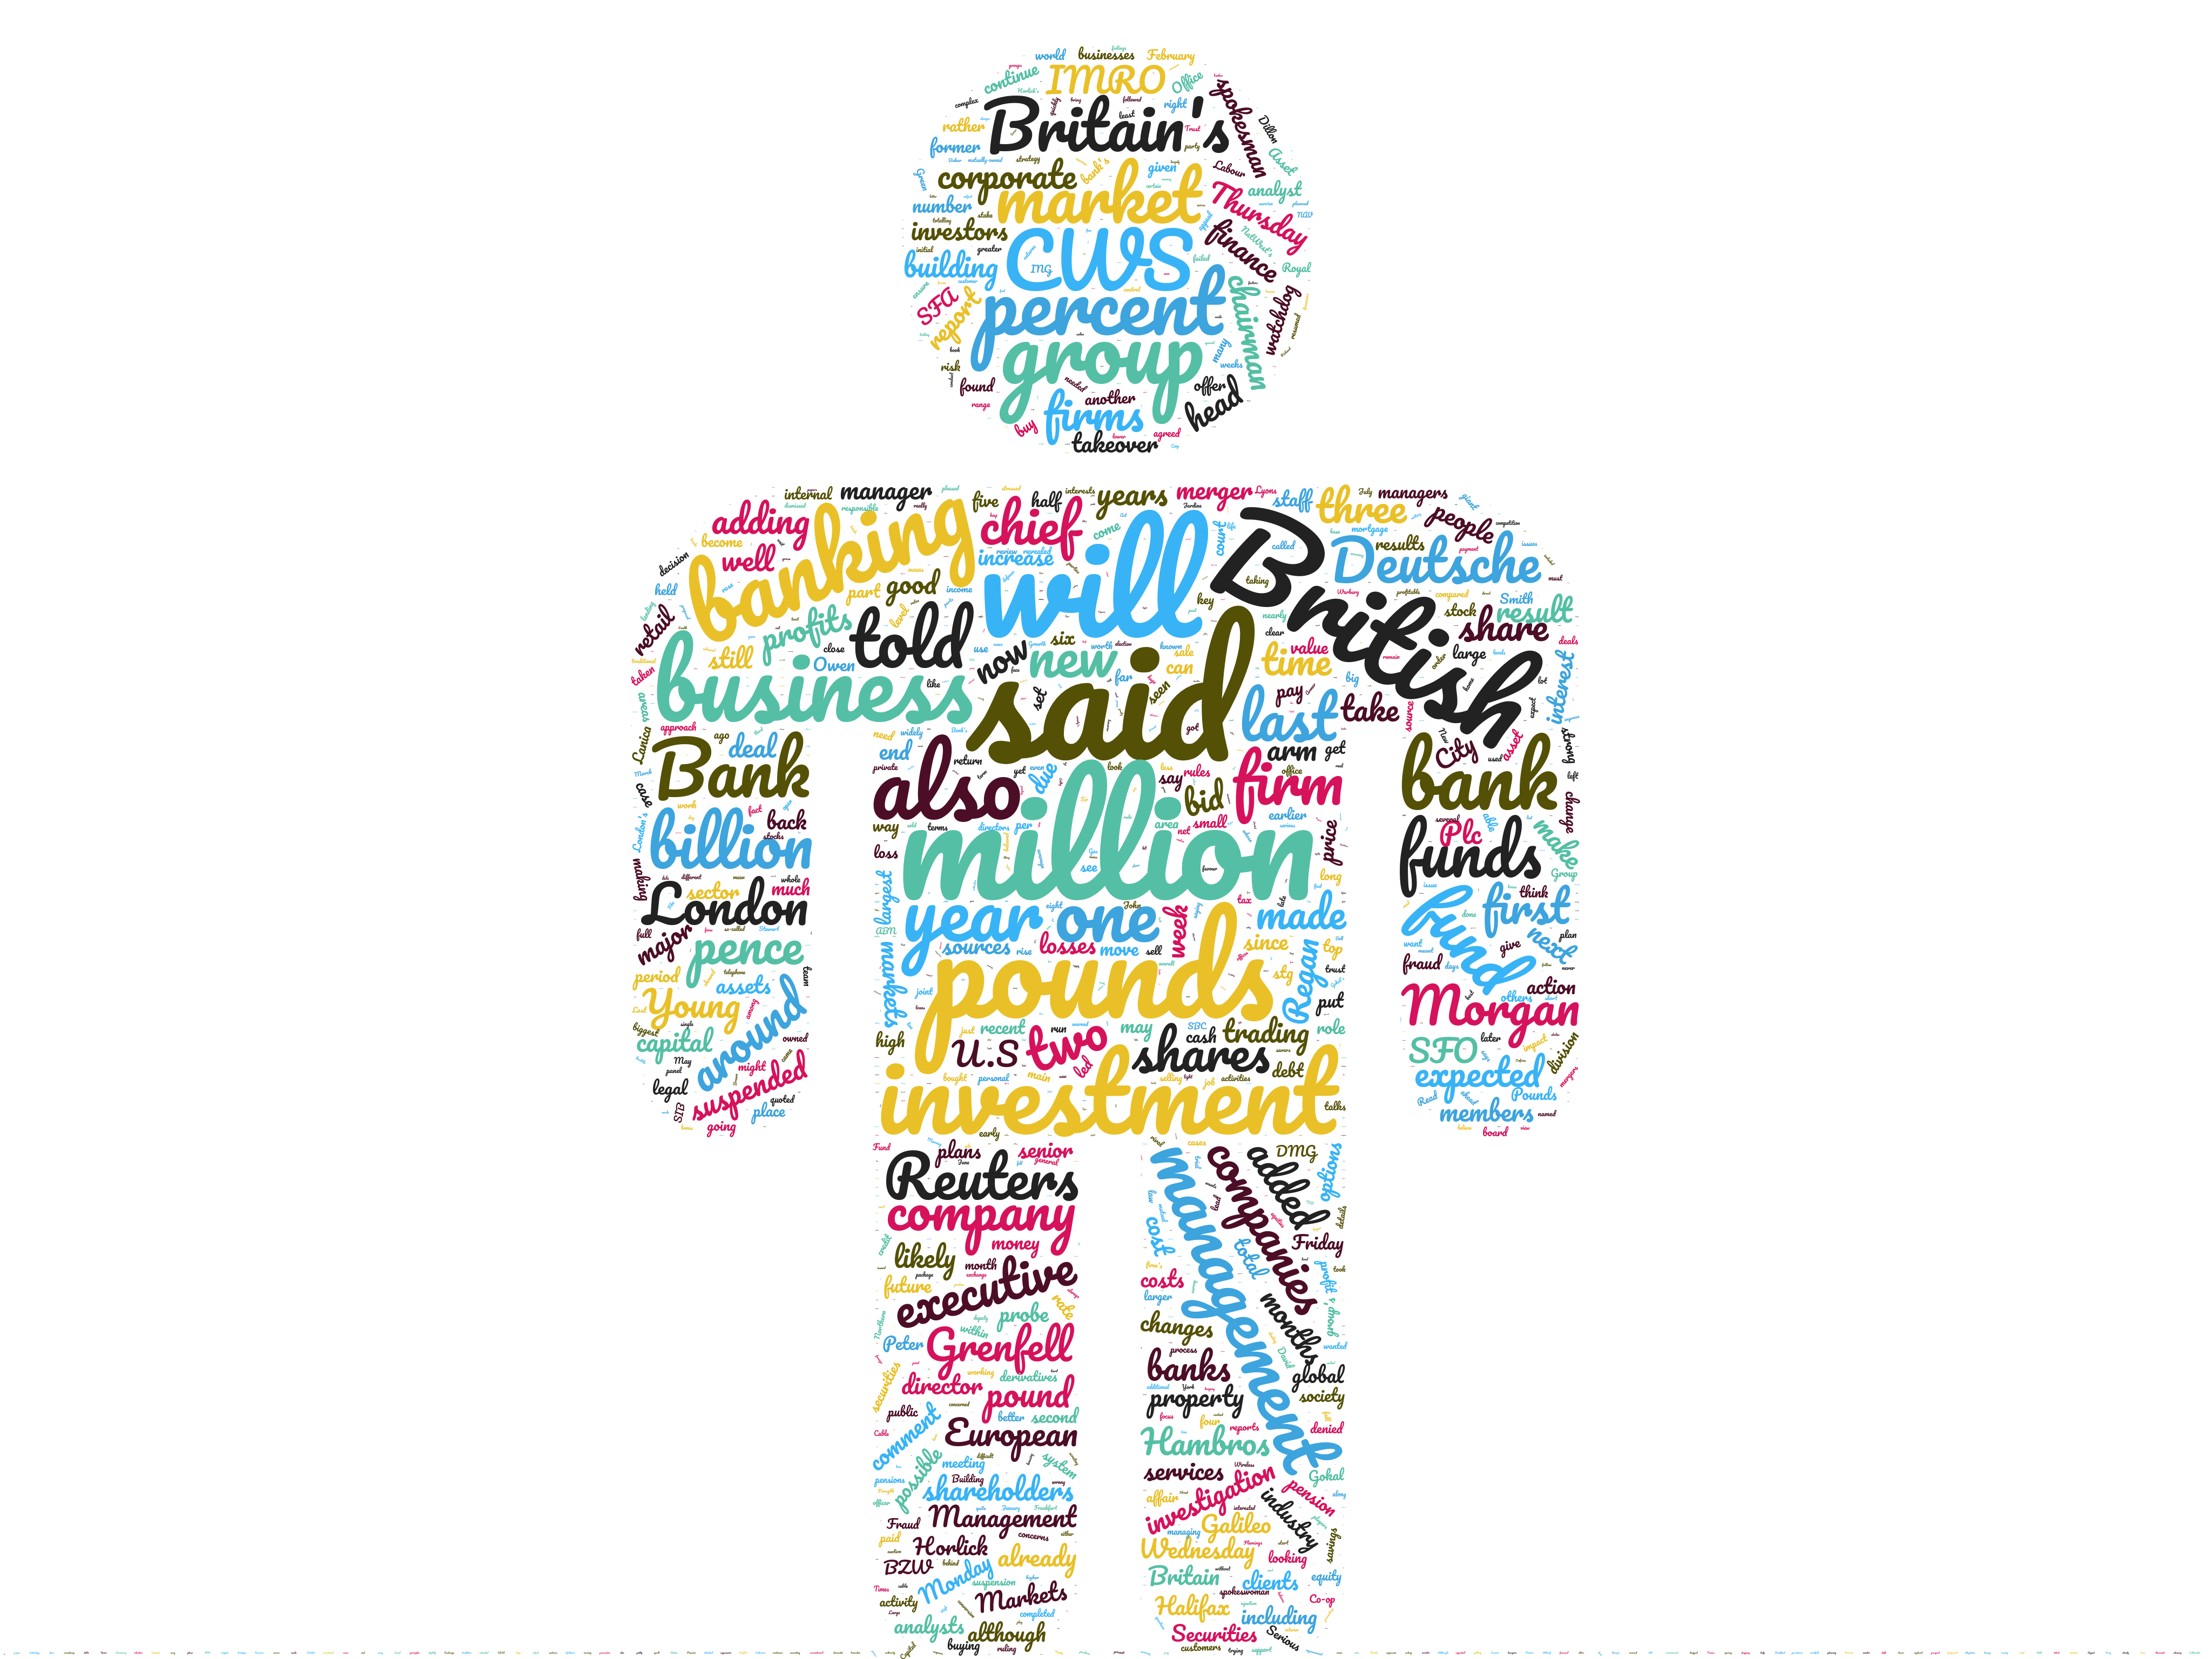
\includegraphics[width=.8\textwidth, height=.6\textheight, keepaspectratio]{Alexander_Smith_wordcloud}
	\caption[Alexander Smith WordCloud in Reuters Corpus Volume 1]{Image Generated on \href{wordclouds.com} for every word in Reuters Corpus Volume 1 corpus data for the documents written by Alexander Smith.}
	\label{fig:wordcloudAS}
\end{figure}

As expected top words are determiners that every writer uses while constructing an English sentence. For example, for \textit{David Lawder} top 20 words are \textit{"the, to, of, and, a, in, said, that, for, GM, on, at, its, The, with, is, it, will, by, from"} but for \textit{Alexander Smith} they are \textit{\enquote{the, of, to, and, a, in, said, was, for, on, it, had, by, be, its, is, with, would, that, as}} in decreasing order. Even though the two sets are mostly the same, the orders and the frequency are different for most authors.

The main assumption with authorship attribution problems is that every authors word usage and content differs and based on these differences the work of one author can be differentiated from the other. In order to illustrate this assumption, in \autoref{fig:chartRCV1ALvsDL} we can see the top 20 words in the RCV1 corpus in the document written by David Lawder, compared to the same words in the documents of Alexander Smith.

In \autoref{fig:wordcloudDL} \& \autoref{fig:wordcloudAS} we plotted using \href{wordclouds.com} the Word Cloud identikit of David Lawder and Alexander Smith, generated by every document written by them in the RCV1 corpus.


\subsection{Word N-grams}
It is a type of probabilistic language model for predicting the next item in the form of a (n-1) order. Considering n-grams are useful since Bag of words miss out the word order when considering a text. For example, a phrasal verb “take on” can be missed out by Bag of words representation which considers “take” and “on” as two separate words. N-gram also establishes the approach of “Skip-gram” language model. An N-gram is a consecutive sub-sequence of length $N$ of some sequence of sentence while a Skip-gram is a N-length sub-sequence where the components occur at a distance of at most $k$ from each other \cite{mikolov2013efficient}.
In order to extract N-grams from a given text data a simple snippet of code is shown in \autoref{lst:MostCommonGrams}, tested for the word grams on the documents written by David Lawder and Alexander Smith of the RCV1 corpus data. No pre-processing on the dataset, such as discarding stopwords, has been done while constructing the N-grams. For David Lawder “the, of the, General Motors Corp.” are the most occurrent uni-gram, bi-gram and 
three-gram respectively whilst in Alexander Smith documents they are “the, of the, said it would”.

\begin{lstlisting}[frame=none,caption={Get the top 3 most common grams in the corpus, for uni-grams, bi-grams and three-grams.},captionpos=b,label=lst:MostCommonGrams]
\end{lstlisting}
\begin{python}	
	from collections import Counter
	from nltk import ngrams
	
	def get_Xigram(text, n):
		"""Get n-grams for a given text. The number of grams are controlled by parameter n"""
		return list(ngrams(text.split(), n))
	
	def get_top_3_gram(df):
		"""Return a list of three elements, each one containing the top 3 most common grams in the corpus given as a Dataframe parameter. The three elements corresponds to the uni-gram, bi-grams and three-grams."""
		result = []
		for i in range(1,4):
			result.append(Counter(get_Xigram(" ".join(df["articles"]), i)).most_common(3))
		return result
	
	print(get_top_3_gram(df_david_lawder))
	print(get_top_3_gram(df_alexander_smith))	
\end{python}


\begin{table}[h!]
	\begin{center}  
		\caption[Top 3 n-grams in Reuters Corpus]{Top 3 uni-grams, bi-grams and three-grams by David Lawder and Alexander Smith in the Reuters corpus data.} 
		\label{tab:tableNGramsRCV1}
		%\resizebox{\linewidth}{!}{  %
		\begin{tabular}{|c | c | c | c|}
			\hline 
			Author & Uni-gram & Bi-gram & Three-gram \\
			\hline \hline
			David Lawder & the & of the & General Motors Corp. \\ \hline
			David Lawder & to & in the	& United Auto Workers \\ \hline
			David Lawder & of & for the	& Ford Motor Co. \\ \hline
			Alexander Smith & the & of the & said it would \\ \hline
			Alexander Smith & of & in the	& the end of \\ \hline
			Alexander Smith & to & said the	& a result of \\ \hline
			%\bottomrule 
		\end{tabular} 
		%}
	\end{center}
\end{table}

Table \ref{tab:tableNGramsRCV1} contains top 3 uni-grams, bi-grams, three-grams from the authors David Lawder and Alexander Smith.

\subsection{Vocabulary Richness}
It is also referred as vocabulary diversity. It attempts to quantify the diversity of the vocabulary text. It is simply the ratio of $V / N$ where $V$ refers to the total number of unique tokens and $N$ refers to the total number of tokens in the considered texts \cite{stamatatos2009survey}. As an example, we applied this feature to the RCV1 CCAT\_10 dataset\footnote{The top ten most prolific authors in the RCV1 corpus, selecting the documents belonging to the \textit{CCAT} topic}.
A snippet of the code to extract such feature, is shown in \ref{lst:vocabRichNessRCV1CCAT10}.

\begin{lstlisting}[frame=none,caption={Calculate vocabulary richness in Reuters Corpus Volume 1 CCAT\_10 split dataset.},captionpos=b,label=lst:vocabRichNessRCV1CCAT10]
\end{lstlisting}
\begin{python}	
		tmp_df = dataset
		tmp_df["num_unique_words"] = tmp_df["articles"].apply(lambda x: len(set(str(x).split()))/len(str(x).split()))
		
		objects = {}
		for author_i in tmp_df.author.unique():
			objects[author_i] = sum(tmp_df[tmp_df.author==author_i]['num_unique_words'])/len(tmp_df[tmp_df.author==author_i])
		
		plt.bar(range(len(objects)), list(objects.values()), align='center')
		plt.xticks(range(len(objects)), list(objects.keys()))
		ax = plt.gca()
		plt.setp(ax.get_xticklabels(), rotation=30, horizontalalignment='right')
		plt.show()
\end{python}

For this portion of the dataset, has been found the lowest vocabulary richness in \textit{Marcel Michelson} and the highest in \textit{Jim Gilchrist}.
Overall distribution of
vocabulary richness is plotted in Figure \ref{fig:rcv1_ccat10_vocab_richness}.

\begin{figure}[ht]
	\centering
	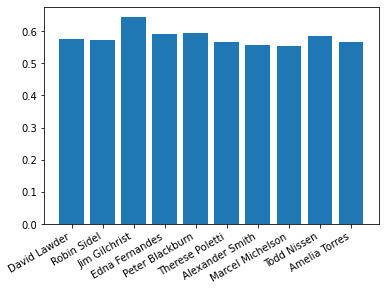
\includegraphics[width=1.0\textwidth, height=1.0\textheight, keepaspectratio]{rcv1_ccat10_vocab_richness}
	\caption[Vocabularity Richness of the Reuters Corpus.]{Bar Plot of vocabulary richness of Reuters Corpus CCAT\_10 authors across all their documents.}
	\label{fig:rcv1_ccat10_vocab_richness}
\end{figure}

\subsection{Stylometric features}

These are features such as number of sentences in a text piece, number of words in a text piece, average number of words in a sentence, average word length in a text piece, number of periods, number of exclamation marks, number of commas, number of colons, number of semicolons, number of incomplete sentences, number of uppercase, title case, camel case, lower case letters. We computed these features comparing the stylometric differences for the documents belonging to David Lawder and the ones of Alexander Smith in the RCV1 corpus. Overall distribution of some of the features introduced here (such as: \textit{number of punctuation, number of words upper case, number of words title, average length of the word, number of stopwords}) are applied and the resulting density measures are calculated for each of the two authors and shown in Table \ref{tab:stylometricFeatRCV1}. Among these five features introduced, number of punctuations and number of stop words usage varies the most among the authors and hence they can be better distinguisher comparing to other feature sets.

\begin{table}[h!]
	\begin{center}  
		\caption[Comparing stylometric features of 2 authors in Reuters Corpus]{Comparing some stylometric features between David Lawder and Alexander Smith calculated on the documents in the Reuters corpus data and normalized by the number of documents.} 
		\label{tab:stylometricFeatRCV1}
		%\resizebox{\linewidth}{!}{  %
		\begin{tabular}{|c | c | c |}
			\hline 
			Stylometric Feature & David Lawder & Alexander Smith \\
			\hline \hline
			Number of punctuation symbols & 101.7800 & 88.7300 \\ \hline
			Number of uppercase words & 12.5900  & 9.8900 \\ \hline
			Number of title words & 76.5900 & 68.3000 \\ \hline
			Word length mean & 5.0900 & 5.1100 \\ \hline
			Number of stopwords & 191.3800 & 234.9700 \\ \hline
			%\bottomrule 
		\end{tabular} 
		%}
	\end{center}
\end{table}

\subsection{Function Words}

Function words are the words that have little meaning on their own but they’re necessary to construct a sentence in English language. They express grammatical relationships among other words within a sentence, or specify the attitude or mood of the speaker. Some of the examples of function words might be prepositions, pronouns, auxiliary verbs, conjunctions, grammatical articles. Words that are not functions words are called as content words and they can also be studied to further analysis the use case in the authorship attribution problems. The search for a single invariant measure of textual style
was natural in the early stages of stylometric analysis, but with the development of more sophisticated multivariate analysis techniques, larger sets of features could be considered.
Among the earliest studies to use multivariate approaches was that of Mosteller and Wallace (1964), who considered distributions of FWs. The reason for using FWs in preference to others is that we do not expect their frequencies to
vary greatly with the topic of the text, and hence, we may hope to recognize texts by the same author on different topics. It also is unlikely that the frequency of FW use can be
consciously controlled, so one may hope that use of FWs for attribution will minimize the risk of being deceived \cite{chung2007psychological}.
Many studies since that of Mosteller and Wallace (1964) have shown the efficacy of FWs for authorship attribution in different scenarios \cite{argamon2005measuring}, \cite{baayen2002experiment}, 
\cite{koppel2005determining},
\cite{zhao2005effective}, confirming the hypothesis that different authors tend to have different characteristic patterns of FW use.
Typical modern studies using FWs in English use lists of a few hundred words, including pronouns, prepositions, auxiliary and modal verbs, conjunctions, and determiners.
Numbers and interjections are usually included as well since they are essentially independent of topic, although they are not, strictly speaking, FWs. Results of different studies using
somewhat different lists of FW have been similar, indicating that the precise choice of FW is not crucial. Discriminators built from FW frequencies often perform at levels competitive with those constructed from more complex features.

\subsection{Term Frequency - Inverse Document Frequency}

It stands for term frequency-inverse document frequency. It is often used as a weight in feature extraction techniques. The reason why Tf-Idf is a good feature can be explained in an example. Let’s assume that a text summarization needs to be done using few keywords. One strategy is to pick the most frequently occurring
terms meaning words that have high term frequency (\textit{tf}). The problem here is that, the most frequent word is a less useful metric since some words like ’a’, ’the’ occur very frequently across all documents. Hence, a measure of how unique a word across all text documents needs to be measured as well (\textit{idf}). Hence, the product of \textit{tf} x \textit{idf} (\ref{TFIDF}) of a word gives a measure of how frequent this word is in the document multiplied by how unique the word is with respect to the entire corpus of documents. Words with a high tf-idf score are assumed to provide the most information about that specific text \cite{stamatatos2009survey}.
\begin{equation}\label{TF}
		TF(t) = \frac{\text{Number of times term t appears in a document}}{\text{Total numbers of terms in the document}}
\end{equation}

\begin{equation}\label{IDF}
	IDF(t) = log_e(\frac{\text{Total number of documents}}{\text{Number of documents with term t in it}}) 
\end{equation}

\begin{equation}\label{TFIDF}
	Tf - Idf = TF(t) * IDF(t)
\end{equation}
As an example, we built a Tf-Idf model by considering documents alone within the text corpus for the authors David Lawder and Alexander Smith.
In the model, not only the single forms of word tokens but their n-grams are considered as well. Table \ref{tab:tableTFIDFRCV1} provides the top 5 words with highest Tf-Idf scores for the two authors. Comparing between Table \ref{tab:tableNGramsRCV1} and Table \ref{tab:tableTFIDFRCV1} new meaningful words have appeared that could serve as a new feature for each author such as “dow, kmart, coupe” for David Lawder or “hsbc, pensions, panel” for Alexander Smith.

\begin{table}[h!]
	\begin{center}  
		\caption[Top 5 Term Frequency - Inversed Document Frequency n-grams in Reuters corpus]{Top 5 Term Frequency - Inversed Document Frequency words n-grams by David Lawder and Alexander Smith in the Reuters Corpus data.} 
		\label{tab:tableTFIDFRCV1}
		%\resizebox{\linewidth}{!}{  %
		\begin{tabular}{|c | c | c || c | c | c |}
			\hline 
			Author & Token & Value & Author & Token & Value \\
			\hline \hline
			David Lawder & \textbf{dow} & \textbf{0.7020} & Alexander Smith & \textbf{hsbc} & \textbf{0.6970} \\ \hline
			David Lawder & kmart & 0.6580	& Alexander Smith & pensions & 0.6010  \\ \hline
			David Lawder & south & 0.5590	& Alexander Smith & bzw & 0.5920 \\ \hline
			David Lawder & coupe & 0.5390 & Alexander Smith & panel & 0.5790 \\ \hline
			David Lawder & bags & 0.5170 & Alexander Smith & read & 0.5700 \\ \hline
			%\bottomrule 
		\end{tabular} 
		%}
	\end{center}
\end{table}


\section{Syntactic Features}

For certain text grammatical and syntactic features could be more useful compared to lexical or character level features. However, this kind of feature extraction techniques requires specific usage of Part of Speech taggers. Some of these features consider the frequency of nouns, adjectives, verbs, adverbs, prepositions, and tense information (past tense,etc). The motivation for extracting these features is that authors tend to use similar syntactic patterns unconsciously \cite{stamatatos2009survey}.
Some researchers are also interested in exploring different dialects of the same language and building classifiers based on features derived from syntactic characteristic of the text. One great example is the work that aims to discriminate between texts written in either the Netherlandic or the Flemish variant of the Dutch language \cite{van2017exploring}.
The feature set in this case consists of lexical, syntactic and word-n grams build on different classifiers and F1 has been recorded for each cases.\\
Employed syntactic features are function words ratio, descriptive words to nominal words ratio personal pronouns ratio, question words ratio, question mark ratio, exclamation
mark ratio \cite{van2017exploring}.

\section{Semantic Features}
Features that we discussed so far aim at analyzing the structural concept of a text. Semantic feature extraction from text data is a bit challenging. That might
explain why there is limited work in this area. One example is the work of Yang who
has proposed combination of lexical and semantic features for short text classification
\cite{yang2013combining}. Their approach consists of choosing a broader domain related to target categories
and then applying topic models such as \textit{Latent Dirichlet Allocation} to learn a certain
number of topics from longer documents. The most discriminative feature words
of short text are then mapped to corresponding topics in longer documents \cite{yang2013combining}.
Their experimental results show significant improvements compared to other related
techniques studying short text classification.
Positivity, neutrality, and negativity index, and synonym usage preference are
good examples of semantic features. Distributed representation of words, Word2Vec,
is also an attempt to extract and represent the semantic features of a word, sentence,
and paragraph \cite{mikolov2010recurrent}. The usage of Word2Vec in authorship attribution tasks has not
yet been studied explicitly. Due to the application domain dependency of Word2Vec
features their usage will be introduced when discussing application specific feature
sets.

\subsection{Positivity and Negativity index}
In order to understand the general mood and the preference of positive and negative sentence structure in each author’s work, a positivity and negativity score has been calculated for the authors \textit{David Lawder} and \textit{Alexander Smith} for the documents in the RCV1 corpora.
The code is shown in \autoref{lst:posnegRCV1CCAT10}, whereas in \autoref{fig:rcv1_ccat10_sentiment_analysis} we can see the results that points out Alexander Smith writing more negative articles than David Lawder. Both of the authors wrote the majority of the articles classified as positive than negative.

\begin{lstlisting}[frame=none,caption={Compute sentence Positivity and Negativity scores.},captionpos=b,label=lst:posnegRCV1CCAT10]
\end{lstlisting}
\begin{python}	
	from nltk.sentiment.vader import SentimentIntensityAnalyzer
	nltk.download('vader_lexicon')
	# Pre-Processing
	SIA = SentimentIntensityAnalyzer()
	# Applying Model, Variable Creation
	sentiment = pd.concat([df_david_lawder, df_alexander_smith])
	sentiment['polarity_score']=sentiment.articles.apply(lambda x:SIA.polarity_scores(x)['compound'])
	sentiment['neutral_score']=sentiment.articles.apply(lambda x:SIA.polarity_scores(x)['neu'])
	sentiment['negative_score']=sentiment.articles.apply(lambda x:SIA.polarity_scores(x)['neg'])
	sentiment['positive_score']=sentiment.articles.apply(lambda x:SIA.polarity_scores(x)['pos'])
	sentiment['sentiment']=''
	sentiment.loc[sentiment.polarity_score>0,'sentiment']='POSITIVE'
	sentiment.loc[sentiment.polarity_score==0,'sentiment']='NEUTRAL'
	sentiment.loc[sentiment.polarity_score<0,'sentiment']='NEGATIVE'
	# Normalize for Size
	auth_sent= sentiment.groupby(['author','sentiment'])[['articles']].count().reset_index()
	for x in ['David Lawder', 'Alexander Smith']:
	auth_sent.articles[auth_sent.author == x] = (auth_sent.articles[auth_sent.author == x]/\
	auth_sent[auth_sent.author ==x].articles.sum())*100
	ax= sns.barplot(x='sentiment', y='articles',hue='author',data=auth_sent)
	ax.set(xlabel='Author', ylabel='Sentiment Percentage')
	ax.figure.suptitle("Author by Sentiment", fontsize = 24)
	plt.show()
\end{python}

\begin{figure}[ht]
	\centering
	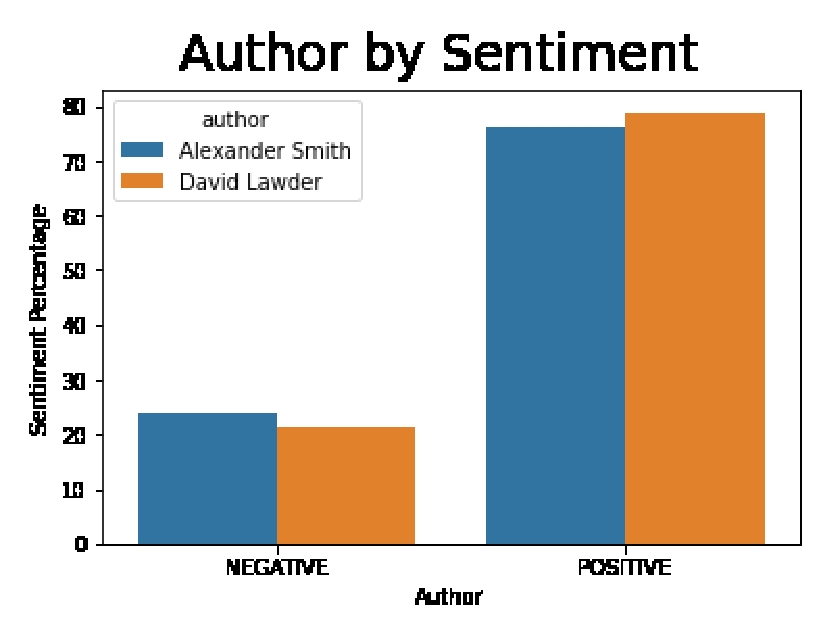
\includegraphics[width=1.0\textwidth, height=1.0\textheight, keepaspectratio]{positivity_negativity_rcv1}
	\caption[Positivity and Negativity scores for Reuters Corpus authors]{Bar Plot of sentiment analysis for 2 of the authors in the Reuters Corpus CCAT\_10 corpora across all their documents.}
	\label{fig:rcv1_ccat10_sentiment_analysis}
\end{figure}

\section{Application Specific Features}

When the application domain of the authorship attribution problems are different
such as email messages or online forum messages, author style can be better characterized using structural, content specific, and language specific features. In such
domains, the use of greetings and farewells, types of signatures, use of indentation,
paragraph lengths, font color, font size could be good features \cite{stamatatos2009survey}.

\subsection{Vector embeddings of words (Word2Vec)}
Word2Vec\footnote{\url{https://code.google.com/archive/p/word2vec/}} leverages the context of the target words. Essentially, we want to use the surrounding words to represent the target words with a Neural Network whose hidden layer encodes the word representation.
Similar words are close
to each other in the vector space. For example, it was shown in \cite{mikolov2013linguistic} that $vector[King] - vector[Man] + vector[Woman]$ results in the vector that is closest to the representation of the $vector[Queen]$.
\autoref{fig:skipgram} shows this representation in a simple way.
The ways to make use of Word2Vec in the dataset is various.
For example, a Word2Vec model can either be built by considering every authors
text data separately, or can be imported using previously trained word vectors on
other large text corpus. It can, then, be plotted into two dimensional vector space
by using dimensionality reduction techniques (TSNE, for example\footnote{t-Distributed Stochastic Neighbor Embedding (t-SNE) is a technique for dimensionality reduction that is particularly well suited for the visualization of high-dimensional datasets}). 
We can also make use of pre-trained word vectors of
Glove to see the difference of usages in such words between an author and a pretrained word vector.
Moving with the idea of training Word2Vec per author, one can also do a cosine
distance measure for the same word or same sentence.
There are two types of Word2Vec, Skip-gram and Continuous Bag of Words (CBOW). I will briefly describe how these two methods work in the following paragraphs.

\begin{figure}[ht]
	\centering
	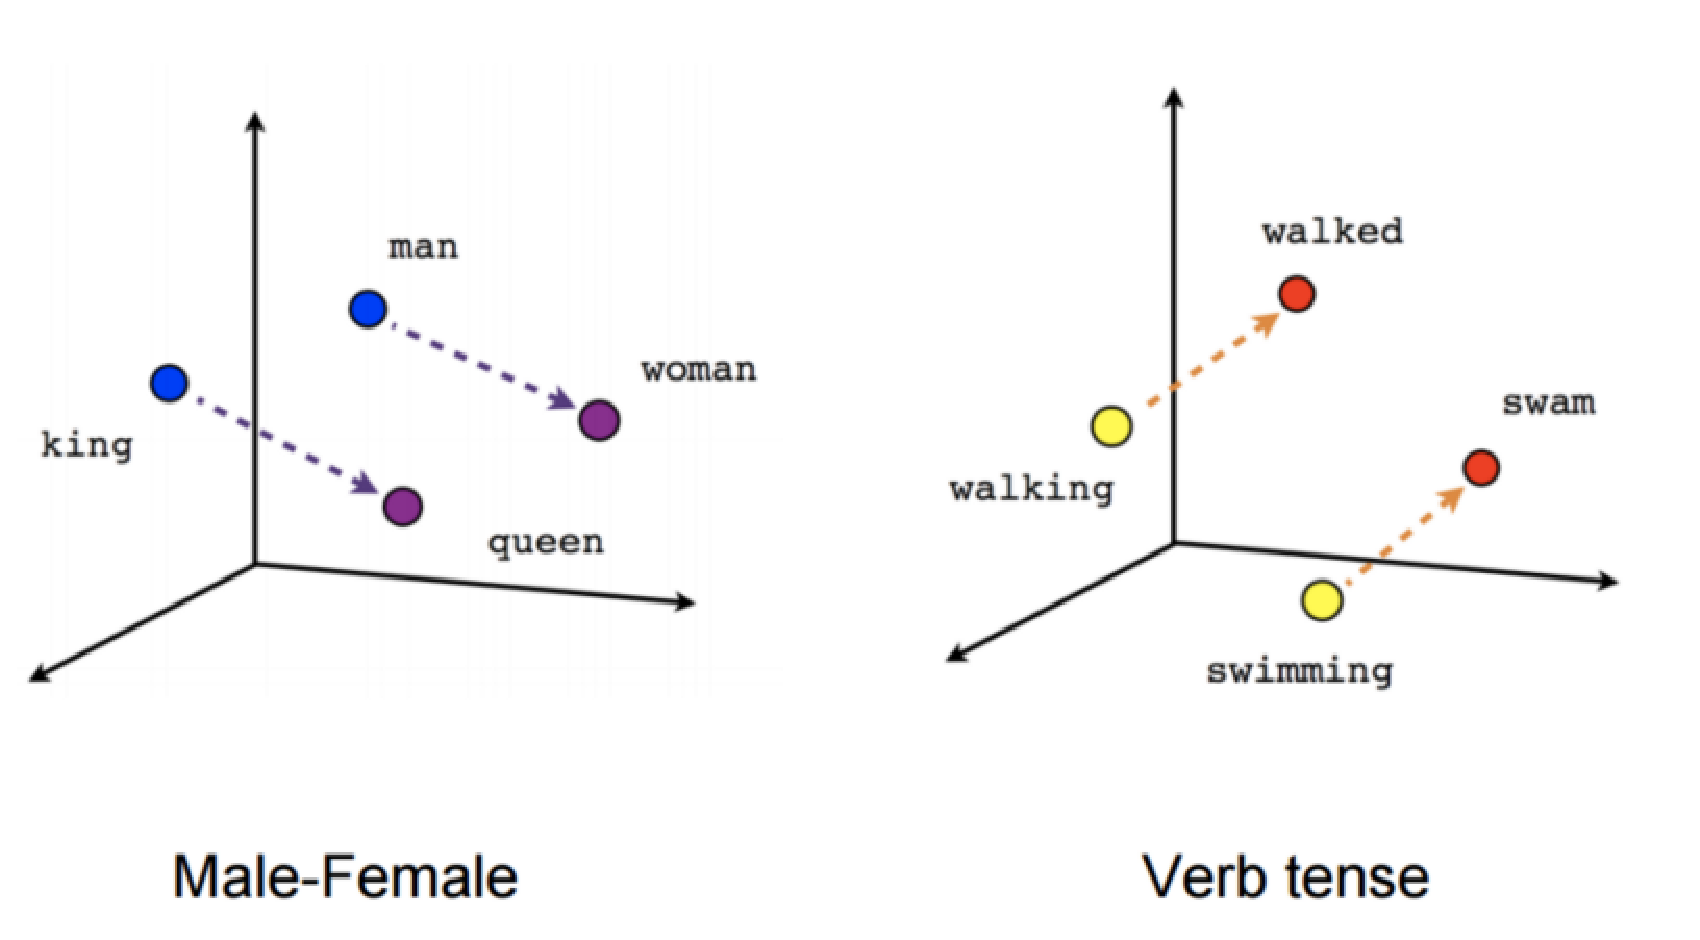
\includegraphics[width=.6\textwidth, height=.6\textheight, keepaspectratio]{skip_gram_2}
	\caption[Word embedding vector representation]{Examples of Word2Vec representation with vector distance.}
	\label{fig:skipgram}
\end{figure}

\subsubsection{Skip-gram}

For skip-gram, the input is the target word, while the outputs are the words surrounding the target words. For instance, in the sentence “I have a cute dog”, the input would be “a”, whereas the output is “I”, “have”, “cute”, and “dog”, assuming the window size is 5. All the input and output data are of the same dimension and one-hot encoded. The network contains 1 hidden layer whose dimension is equal to the embedding size, which is smaller than the input/output vector size. At the end of the output layer, a
softmax activation function is applied so that each element of the output vector describes how likely a specific word will appear in the context.
In mathematics, the softmax function, or normalized exponential function is a generalization of the logistic function that \textit{squashes} a K-dimensional vector z of arbitrary real values to a K-dimensional vector $\delta$(z) of real values, where each entry is in the range (0,1) and all the entries add up to 1. The target is a (K-1)-dimensional space, so one dimension has been lost.\\\\
With skip-gram, the representation dimension decreases from the vocabulary size (V) to the length of the hidden layer (N). Furthermore, the vectors are more “meaningful” in terms of describing the relationship between words. The vectors obtained by subtracting two related words sometimes express a meaningful concept such as gender or verb tense, as shown in the following figure (dimensionality reduced).

\subsubsection{Continuous Bag Of Words (CBOW)}

Continuous Bag of Words (CBOW)\footnote{\url{https://iksinc.online/tag/continuous-bag-of-words-cbow/}} is very similar to skip-gram, except that it swaps the input and output. The idea is that given a context, we want to know which word is most likely to appear in it.\\
The biggest difference between Skip-gram and CBOW is that the way the word vectors are generated. For CBOW, all the examples with the target word as target are fed into the networks, and taking the average of the extracted hidden layer. For example, assume we only have two sentences, “He is a nice guy” and “She is a wise queen”. To compute the word representation for the word “a”, we need to feed in these two examples, “He is nice guy”, and “She is wise queen” into the Neural Network and take the average of the value in the hidden layer. Skip-gram only feed in the one and only one target word one-hot vector as input.

It is claimed that Skip-gram tends to do better in rare words. Nevertheless, the performance of Skip-gram and CBOW are generally similar.

\subsection{Vector embeddings of documents (Doc2Vec)}

Distributed word representation in a vector space (word embeddings) is a novel technique that allows to represent words in terms of the elements in the neighborhood.
Distributed representations can be extended to larger language structures like phrases, sentences, paragraphs and documents. The capability to encode semantic information of texts and the ability to handle high-dimensional datasets are the reasons why this representation is widely used in various natural language processing tasks such as text summarization, sentiment analysis and syntactic parsing \cite{le2014distributed}.

\begin{figure}[ht]
	\centering
	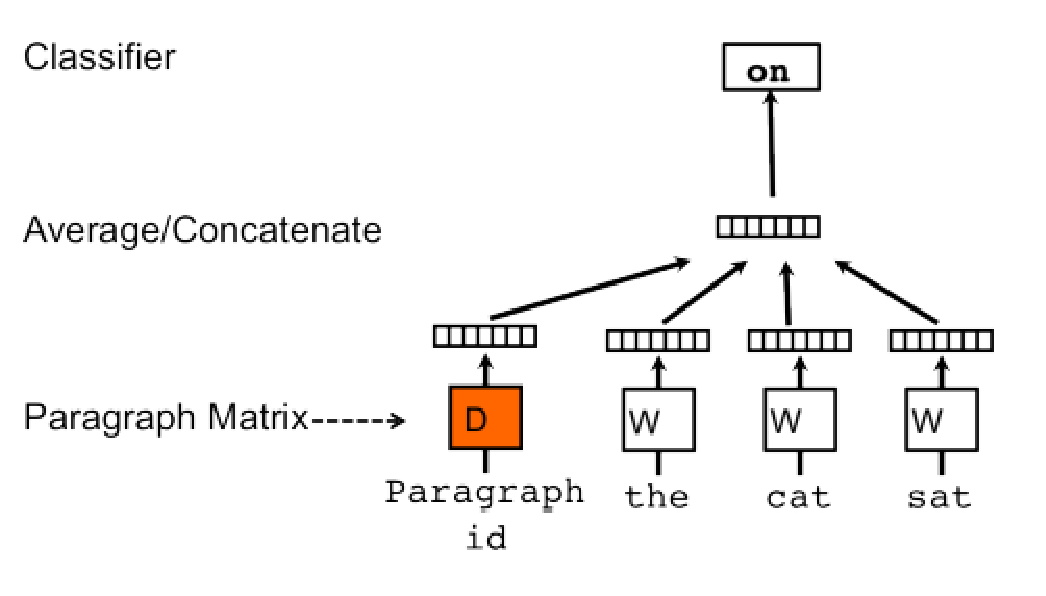
\includegraphics[width=.6\textwidth, height=.6\textheight, keepaspectratio]{dmd2v}
	\caption[Paragraph vector distributed memory model example]{Paragraph Vector-Distributed Memory model.}
	\label{fig:pv-dm}
\end{figure}

The goal of doc2vec is to create a numeric representation of a document, regardless of its length.
Unlike words, documents do not come in logical structures such as words, so the another method has to be found.
The concept that Mikilov and Le \cite{le2014distributed} had used was simple, yet clever: they used the word2vec model, but instead of using just words to predict the next word, we also added another feature vector, which is document-unique.
When training the word vectors W, the document vector D is trained as well, and in the end of training, it holds a numeric representation of the document.

\begin{figure}[ht]
	\centering
	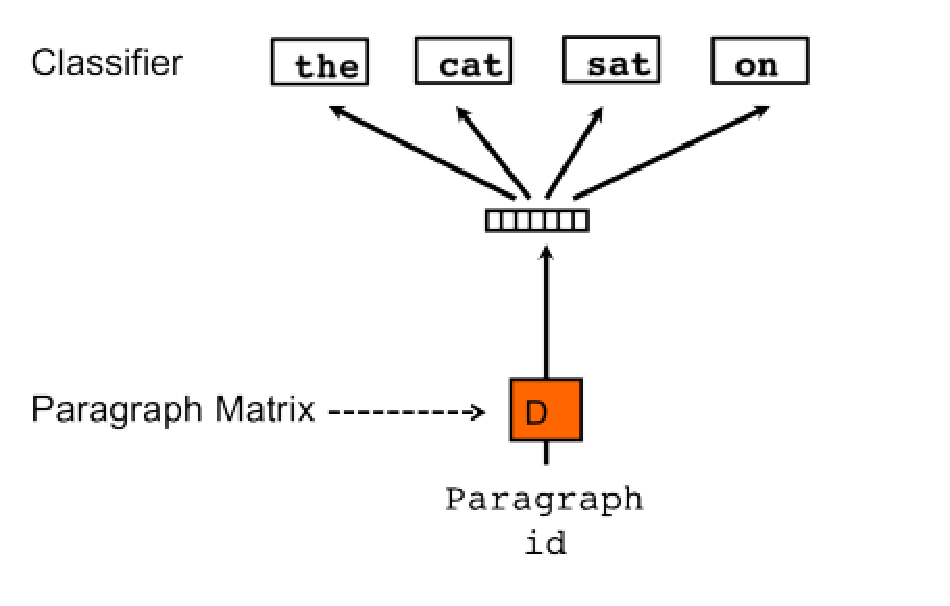
\includegraphics[width=.6\textwidth, height=.6\textheight, keepaspectratio]{dbowd2v}
	\caption[Paragraph vector distributed bag of words model example]{Paragraph Vector-Distributed Bag of Words model.}
	\label{fig:pv-dbow}
\end{figure}

The model above is called \textit{Distributed Memory version of Paragraph Vector} (PV-DM) \autoref{fig:pv-dm}. It acts as a memory that remembers what is missing from the current context — or as the topic of the paragraph. While the word vectors represent the concept of a word, the document vector intends to represent the concept of a document.
As in word2vec, another algorithm, which is similar to skip-gram may be used \textit{Distributed Bag of Words version of Paragraph Vector} (PV-DBOW).
As we can see in \autoref{fig:pv-dbow}, this algorithm is actually faster (as opposed to word2vec) and consumes less memory, since there is no need to save the word vectors.
